\documentclass[12pt,a4paper]{article}
\usepackage[utf8]{inputenc}
\usepackage[T1]{fontenc}
\usepackage{graphicx}
\usepackage{float}
\usepackage{geometry}
\usepackage{fancyhdr}
\usepackage{amsmath}
\usepackage{amsfonts}
\usepackage{amssymb}
\usepackage{xcolor}
\usepackage{listings}
\usepackage{hyperref}
\usepackage{caption}
\usepackage{subcaption}

% Page settings
\geometry{left=2.5cm,right=2.5cm,top=2.5cm,bottom=2.5cm}
\pagestyle{fancy}
\fancyhf{}
\fancyhead[L]{Tutorial 4 - IPTables Firewall Configuration Lab}
\fancyhead[R]{\thepage}

% Code block settings
\lstset{
    basicstyle=\ttfamily\small,
    backgroundcolor=\color{gray!10},
    frame=single,
    breaklines=true,
    showstringspaces=false,
    numbers=left,
    numberstyle=\tiny\color{gray},
    keywordstyle=\color{blue},
    commentstyle=\color{green!60!black},
    stringstyle=\color{red}
}

\title{\textbf{Tutorial 4 Lab Report} \\ IPTables Firewall Configuration Experiment}
\author{Student Name: GuYi}
\date{\today}

\begin{document}

\maketitle

\section{Experiment Objectives}
This experiment aims to learn the configuration and management of iptables firewall in Linux systems through practical operations, including:
\begin{itemize}
    \item Understanding the basic concepts and working principles of iptables
    \item Mastering the creation, modification, and deletion of firewall rules
    \item Learning control methods for different types of network traffic
    \item Understanding the priority and matching mechanisms of firewall rules
    \item Practicing the implementation of network security protection strategies
\end{itemize}

\section{Experiment Environment}
\begin{itemize}
    \item Operating System: Linux (Ubuntu/CentOS)
    \item Firewall Tool: iptables
    \item Testing Tools: ping, curl, nslookup, netcat, etc.
    \item Virtual Machine Environment: Safe experimental environment
\end{itemize}

\section{Experiment Steps and Results}

\subsection{Preparation Phase - Environment Cleanup}

Before starting the experiment, we need to clean up existing iptables rules to ensure we start from a clean state. This involves switching to root user, backing up current rules, cleaning all existing rules, and setting permissive policies for all chains.

\begin{figure}[H]
    \centering
    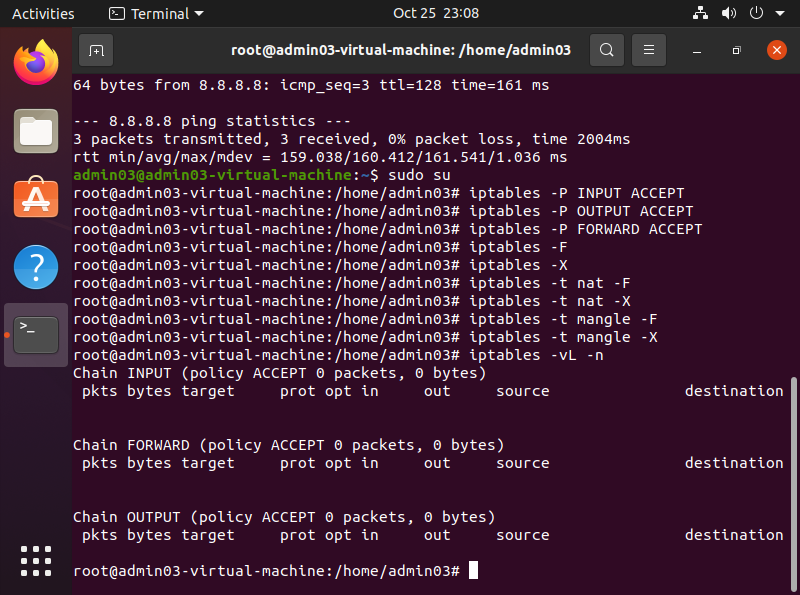
\includegraphics[width=0.9\textwidth]{02_clean_iptable.png}
    \caption{IPTables state after cleanup - showing all chains are empty with ACCEPT policy}
    \label{fig:clean_iptables}
\end{figure}

From Figure \ref{fig:clean_iptables}, we can see that after cleanup, iptables shows that all three main chains (INPUT, FORWARD, OUTPUT) have no rules, and the default policies are all set to ACCEPT, providing a clean starting environment for subsequent experiments.

\subsection{Rule 1: Setting Default Policies}

Setting the default policy of the firewall is the first step in firewall configuration, usually adopting a "default deny" security strategy. We set the INPUT chain default policy to DROP (deny) and OUTPUT chain default policy to ACCEPT (allow).

\begin{figure}[H]
    \centering
    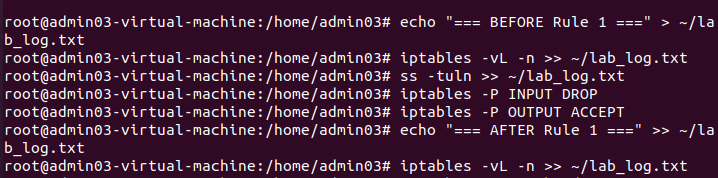
\includegraphics[width=0.9\textwidth]{03_default_policy.png}
    \caption{IPTables state after setting default policies - INPUT policy is DROP, OUTPUT policy is ACCEPT}
    \label{fig:default_policy}
\end{figure}

Figure \ref{fig:default_policy} shows the state after setting default policies. The INPUT chain policy becomes DROP, meaning all inbound traffic is denied by default; the OUTPUT chain remains ACCEPT, allowing all outbound traffic. This is a common security configuration strategy.

\subsection{Rule 2: Allow Loopback Communication}

The loopback interface is used for internal machine communication and must remain open to ensure normal system operation. We configure rules to allow both inbound and outbound traffic on the loopback interface and test the communication.

\begin{figure}[H]
    \centering
    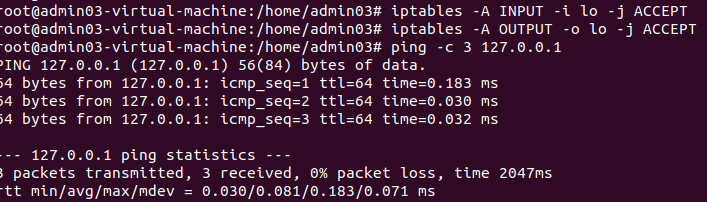
\includegraphics[width=0.9\textwidth]{04_loopback_rule.png}
    \caption{Loopback interface rule configuration and test results}
    \label{fig:loopback_rule}
\end{figure}

Figure \ref{fig:loopback_rule} shows the configuration results of loopback interface rules. We can see that two new rules have been added to iptables, allowing inbound and outbound traffic on the loopback interface respectively. The ping test results show that local loopback communication works normally.

\subsection{Rule 3: Allow ICMP Protocol}

ICMP protocol is used for network diagnostics and error reporting, including the commonly used ping command. We configure rules to allow both inbound and outbound ICMP traffic and test ping to external networks.

\begin{figure}[H]
    \centering
    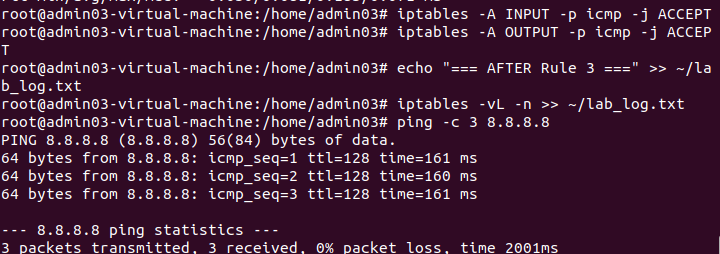
\includegraphics[width=0.9\textwidth]{05_icmp_rul.png}
    \caption{ICMP protocol rule configuration and ping test results}
    \label{fig:icmp_rule}
\end{figure}

Figure \ref{fig:icmp_rule} shows the state after ICMP rule configuration. Rules allowing ICMP protocol have been added to iptables, and the ping test to 8.8.8.8 was successful, proving that ICMP traffic can pass through the firewall normally.

\subsection{Rule 4: Allow Outbound Web Access}

Configure outbound access for HTTP and HTTPS protocols, which is a basic requirement for modern network applications. We allow outbound connections on ports 80 and 443, and configure corresponding inbound rules for established connections using state tracking.

\begin{figure}[H]
    \centering
    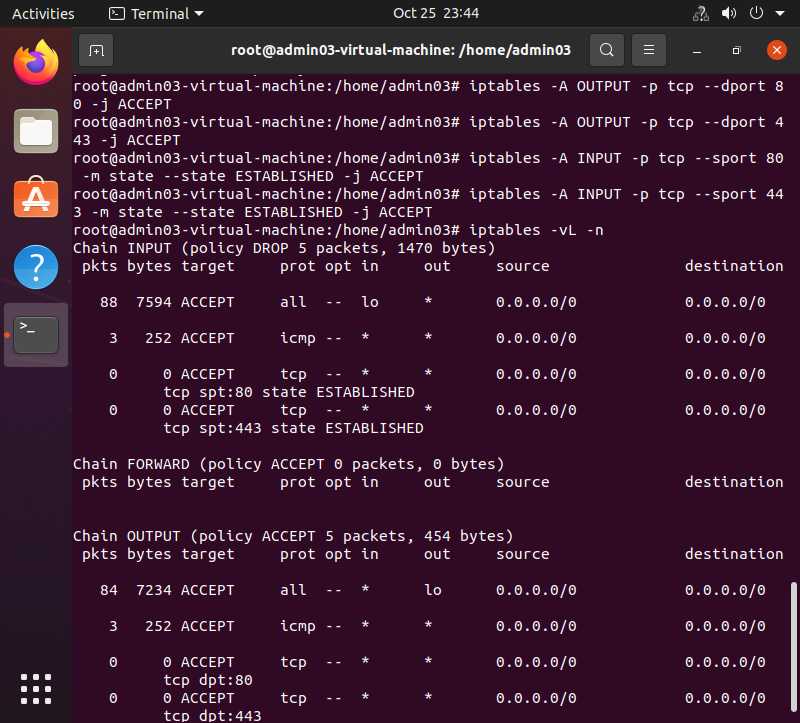
\includegraphics[width=0.9\textwidth]{06_web_access_rule.png}
    \caption{Web access rule configuration results}
    \label{fig:web_access_rule}
\end{figure}

Figure \ref{fig:web_access_rule} shows the configuration of web access rules. We can see four new rules have been added, handling HTTP and HTTPS outbound requests and their corresponding inbound responses. The state tracking mechanism (state ESTABLISHED) is used to allow response packets from established connections.

\subsection{Rule 5: Enable DNS Resolution}

DNS resolution is the foundation of network access, requiring configuration of access rules for UDP port 53. We allow DNS queries and test both DNS resolution and web access functionality.

\begin{figure}[H]
    \centering
    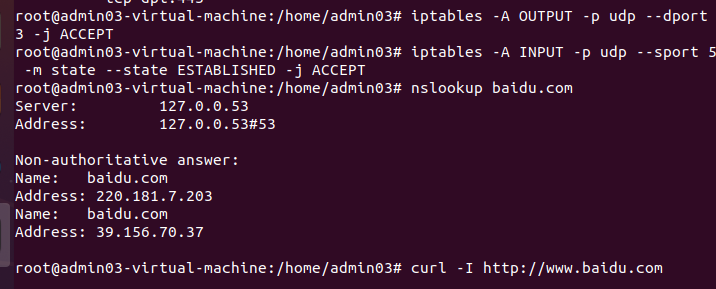
\includegraphics[width=0.9\textwidth]{07_dns_rule.png}
    \caption{DNS rule configuration and test results}
    \label{fig:dns_rule}
\end{figure}

Figure \ref{fig:dns_rule} shows the test results after DNS rule configuration. The nslookup command successfully resolved the baidu.com domain name, and the curl command was also able to access the website normally, indicating that both DNS resolution and web access functions work properly.

\subsection{Rule 6: Block Specific Website Access}

Demonstrate how to block access to specific websites, which is a basic implementation of content filtering. We find the IP address of the target website, block access to that specific IP, and test the blocking effect.

\begin{figure}[H]
    \centering
    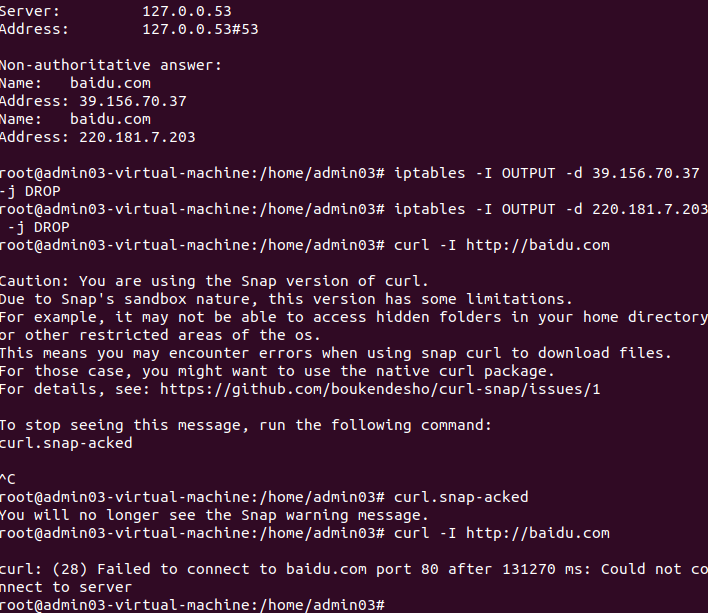
\includegraphics[width=0.9\textwidth]{08_block_websit.png}
    \caption{Website blocking rule configuration and test results}
    \label{fig:block_website}
\end{figure}

Figure \ref{fig:block_website} shows the implementation of website blocking functionality. We obtained the IP address of facebook.com through nslookup, then used iptables rules to block access to that IP. Test results show that access to facebook.com is blocked, while access to baidu.com remains normal.

\subsection{Rule 7-8: Complete Rule Configuration}

Add support for other commonly used protocols, such as SSH. We allow outbound SSH connections and configure corresponding inbound rules for established connections, then view the complete rule configuration.

\begin{figure}[H]
    \centering
    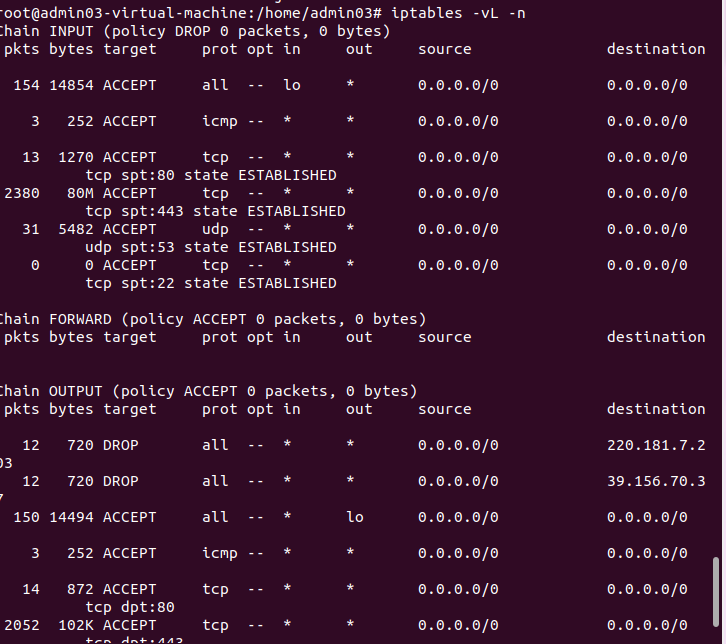
\includegraphics[width=0.9\textwidth]{09_complete_rules.png}
    \caption{Complete firewall rule configuration}
    \label{fig:complete_rules}
\end{figure}

Figure \ref{fig:complete_rules} shows the complete firewall rule configuration. We can see that the INPUT chain contains rules for loopback, ICMP, web responses, DNS responses, and SSH responses; the OUTPUT chain contains rules for loopback, ICMP, web requests, DNS requests, SSH requests, and website blocking.

\subsection{Rule 9: Inbound Web Service Configuration}

Configure web server to allow external access to the local web service. We install Apache web server, allow inbound HTTP access, start the Apache service, and test the local web service.

\begin{figure}[H]
    \centering
    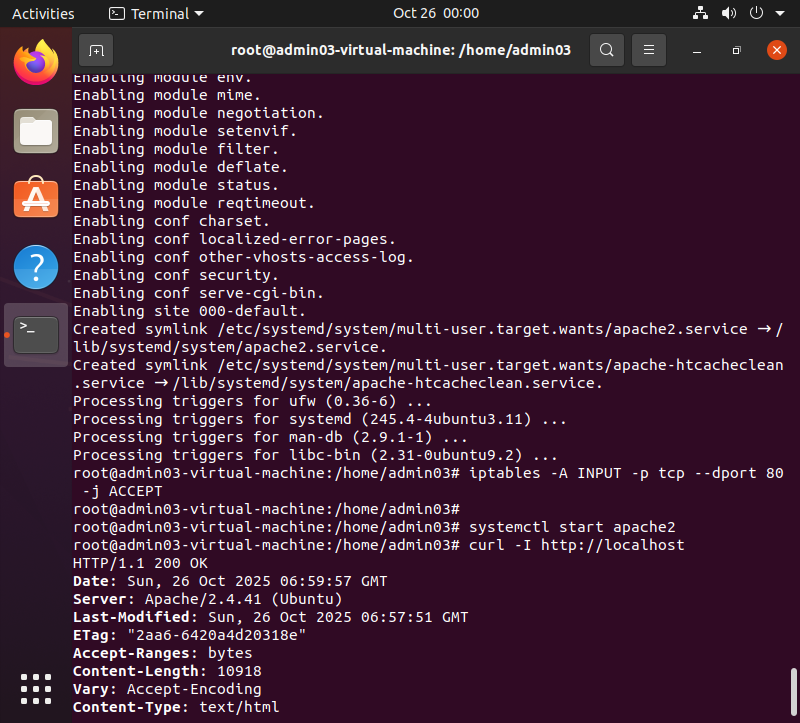
\includegraphics[width=0.9\textwidth]{10_inbound_web.png}
    \caption{Inbound web service configuration and testing}
    \label{fig:inbound_web}
\end{figure}

Figure \ref{fig:inbound_web} shows the configuration process of inbound web service. The Apache server was successfully installed and started, iptables rules allow inbound HTTP connections, and the curl test shows that the local web service responds normally.

\subsection{Rule 10: Rule Priority Testing}

Demonstrate the priority mechanism of iptables rules, where the first matching rule determines packet processing. We add conflicting rules to test priority, view the rule order, and test port access.

\begin{figure}[H]
    \centering
    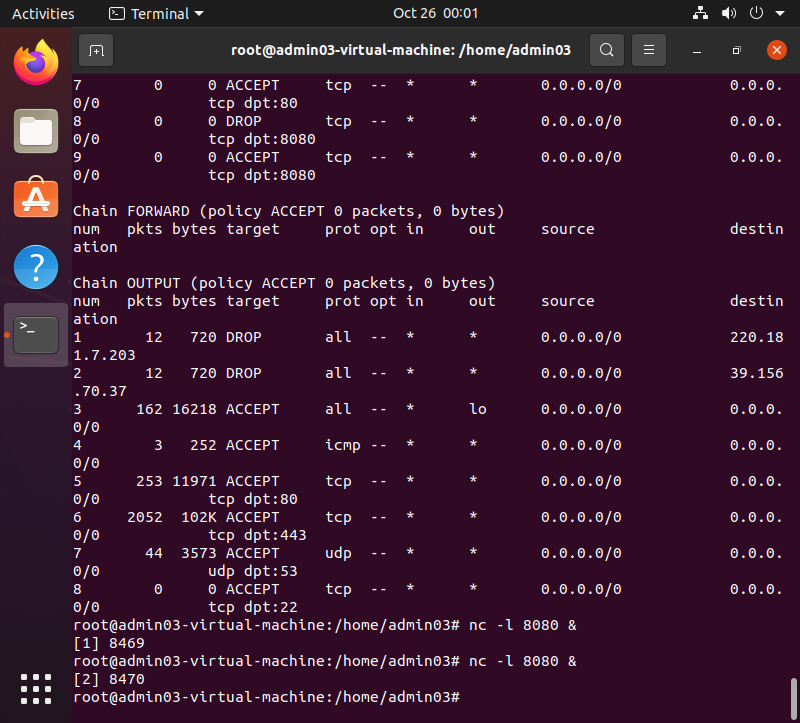
\includegraphics[width=0.9\textwidth]{11_rule_priority.png}
    \caption{Rule priority test results}
    \label{fig:rule_priority}
\end{figure}

Figure \ref{fig:rule_priority} demonstrates the priority mechanism of iptables rules. Two conflicting rules were added: first DROP then ACCEPT for the same port. Since iptables matches rules in order, the first DROP rule takes effect, and the subsequent ACCEPT rule is not executed.

\subsection{Final Configuration Check}

View the final complete firewall configuration state. We examine the final complete rules with line numbers and view rule statistics.

\begin{figure}[H]
    \centering
    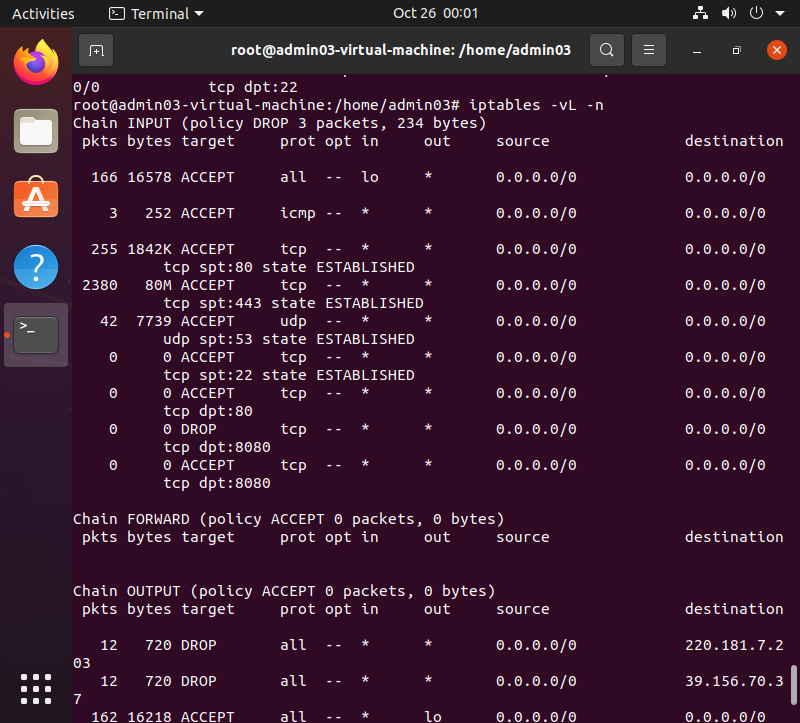
\includegraphics[width=0.9\textwidth]{12_final_configuration.png}
    \caption{Final complete firewall configuration}
    \label{fig:final_configuration}
\end{figure}

Figure \ref{fig:final_configuration} shows the final firewall configuration after completing the experiment. We can see the complete rule set, including support for various protocols, website blocking, service access control, and other functions. Rule statistics show the match count and traffic statistics for each rule.

\section{Experiment Summary and Analysis}

\subsection{Experiment Achievements}
Through this experiment, the following tasks were successfully completed:
\begin{enumerate}
    \item \textbf{Basic Configuration}: Mastered basic iptables operations, including rule cleanup, policy setting, etc.
    \item \textbf{Protocol Control}: Learned to configure access rules for different network protocols (ICMP, HTTP, HTTPS, DNS, SSH)
    \item \textbf{Access Control}: Implemented website blocking functionality, understanding IP address-based access control
    \item \textbf{Service Configuration}: Configured inbound access rules for web servers
    \item \textbf{Rule Priority}: Understood the matching order and priority mechanism of iptables rules
\end{enumerate}

\subsection{Key Technical Points}
\begin{itemize}
    \item \textbf{Default Policy}: Adopting "default deny" policy to improve security
    \item \textbf{State Tracking}: Using connection tracking mechanism to manage connection states
    \item \textbf{Rule Order}: IPTables matches rules in order, the first matching rule determines processing
    \item \textbf{Port Control}: Controlling different types of network traffic through source and destination ports
    \item \textbf{Interface Control}: Using network interface parameters to control traffic on specific interfaces
\end{itemize}

\subsection{Security Considerations}
\begin{itemize}
    \item Loopback interface must remain open, otherwise internal system communication will be affected
    \item SSH rule configuration requires caution to avoid locking out remote access
    \item Rule order is important, more specific rules should be placed first
    \item Regularly backup firewall rules for fault recovery
    \item Thorough testing should be conducted before applying rules in production environments
\end{itemize}

\subsection{Experiment Insights}
This experiment gave me a deep understanding of the working principles and configuration methods of Linux firewalls. IPTables, as an important security component of Linux systems, provides powerful protection for network security through its flexibility and powerful functionality. Through practical operations, I mastered the design concepts and implementation methods of firewall rules, which is of great significance for system administration and network security work.

The main challenges encountered during the experiment were understanding the rule matching logic and state tracking mechanisms. Through repeated testing and log observation, I finally mastered these key concepts.

\section{References}
\begin{itemize}
    \item Linux iptables Official Documentation
    \item "Linux Firewall Configuration Guide"
    \item Tutorial 4 Lab Guide Document
    \item Network Security Related Technical Materials
\end{itemize}

\end{document}